\section{Optical Distortion Correction}
In this section, we develop optical calibration and distortion correction for our volumetric augmented reality display. An unintended property of this display is that the field-of-view of the depth planes changes slightly over depth. This change in field-of-view can cause the following problems:

\begin{enumerate}
    \item Image distortions: if two digital objects at different depths are expected to line up with each other, they will not. Alternatively, a long object somewhat parallel to the display axis will appear to curve rather than look straight.
    \item Reduced spatial resolution: since some of these displays distribute the decomposition of a color voxel over multiple binary voxels at different depths, the slight curve can introduce a blurring effect and lead to a loss in spatial resolution~\cite{Rathinavel2018}. 
    \item Incorrect depth cues: Some depth cues, e.g., motion parallax, perspective, relative density, and relative size, will be slightly incorrect due to this distortions~\cite{cutting1995perceiving}.
\end{enumerate}

To address these issues, we develop an optical calibration method and a distortion correction as a post-processing step to our rendering pipeline. 

\subsection{Approach for calibration and distortion correction}
\begin{figure} [ht]
\begin{center}
\begin{tabular}{c} 
\includegraphics[width=\textwidth]{images/volumetric/distortion_correction/synthetic}
\end{tabular}
\end{center}
\label{fig:volumetric:distortion_correction:synthetic} 
\caption{(Left) Calibration image that can be placed at multiple depth-planes. (Right) Calibration volume which is mostly composed of fully-black images (depicted by gray border) with a few calibration images (depicted by green border).}
\end{figure} 

Our approach for calibration and distortion correction assumes that the depth-planes are centered on and perpendicular to the display's optical axis. 
The reason we assume this is because it is difficult to measure the depth of one (or a few nearby) display voxels. 
To measure the depth, we would need a camera with a very narrow depth-of-field such that it can discern the difference in depth between any two adjacent depth-planes --- this is not practical. 
Besides, the human vision's depth of field is 0.3 diopters, and our depth-plane spacing is dense enough to be well within the 0.3 diopters threshold~\cite{Rathinavel2018}. Below we discuss each stage of our one-time calibration procedure and our post-rendering distortion correction step.

\subsubsection{Synthetic volume for calibration}
To use in the calibration steps, we generate a synthetic volume composed of mostly black images interspersed with images composed of a centered rectangle, centered horizontal line, and centered vertical line are bright.
An example calibration image is shown in Fig.~\ref{fig:volumetric:distortion_correction:synthetic} (left). This image is placed at a sparse set of depth planes. Fig.~\ref{fig:volumetric:distortion_correction:synthetic} (right) is a concept diagram explaining the sparse locations of the calibration images --- gray bordered depth-planes are fully black images whereas green bordered depth-planes contain the calibration pattern shown in Fig.~\ref{fig:volumetric:distortion_correction:synthetic} (left). Note that unlike the depiction in Fig.~\ref{fig:volumetric:distortion_correction:synthetic} (right), our display's volume is much denser (composed of 280 depth-planes). 

\subsubsection{Pre-calibration: Aligning camera's and display's optical axis}
To demonstrate our calibration and distortion correction, we first need to align the recording camera's axis to coincide with the display's axis. An explanation for this follows:

Recall that in our display, each color voxel is decomposed into some binary voxels such that these binary voxels will lie on a single perspective projection line such that they get integrated onto the same retinal or camera pixel. 
Since multifocal plane displays are view-dependent displays, it is necessary to track the pupil position and the decomposition also needs to be view-dependent.
But, in this paper, we do not use an eye-tracker, and we assume that all the depth planes are centered and perpendicular to the display's optical axis.
If we assume the eye's axis to be aligned with the display's axis, the display's axis is the only line that will not need calibration or distortion correction. Hence, we need to align the camera's and display's axis.

To align the camera's axis with the display's axis, the stack of synthetic images is displayed and the camera's position was manually adjusted until the centered-horizontal and centered-vertical lines aligned. When aligned properly, the image seen is shown in Fig.~\ref{fig:volumetric:distortion_correction:results} (left).

\subsubsection{Calibration}
\label{sec:volumetric:distortion_correction:calibration}
Our calibration approach is to sample the field-of-view for a sparse set of depth-planes and interpolate the scaling factor that needs to be applied to each depth-plane to ensure a constant field-of-view across the entire volume. This happens in these steps:
\begin{figure} [ht]
\begin{center}
\includegraphics[width=\textwidth]{images/volumetric/distortion_correction/scale_v_depth}
\end{center}
\caption[Volumetric NED: Relative scale as a function of depth]{Plot of the relative scale as a function of the depth-plane's index, i.e., $s(j)$ mentioned in Sec.~\ref{sec:volumetric:distortion_correction:calibration}}
\label{fig:volumetric:distortion_correction:scale_v_depth} 
\end{figure} 


\begin{enumerate}
    \item To sample the field-of-view for each depth-plane, we place the image shown in Fig.~\ref{fig:volumetric:distortion_correction:synthetic}(left) at that depth plane, capture the image seen by a camera, and measure the number of pixels between the left edge of the outer rectangle to the right edge of the outer rectangle. Say this results in a set $\{\theta_i\}$ where $\theta_i$ is the field-of-view of the $i^{\text{th}}$ depth-plane and $i \in [1,...,M]$, where $M$ is the number of depth planes where we sample the field-of-view. In our experiment, $M = 10$.
    \item We calculate the relative scaling factor for these depth planes as $s(i) = \frac{\theta_i}{\theta_1}$, i.e., the first (nearest) depth-plane is assumed to have a scaling factor of 1 and all other depth-planes are assumed to be scaled relative to this.
    \item We estimate the scaling factor for all depth-planes as the function $s(j), j \in [1,280]$ as a cubic interpolation of the data-points $\{(s(i), i)\}, i\in [1,M]$. This interpolation is shown in Fig.~\ref{fig:volumetric:distortion_correction:scale_v_depth} where the blue circles are the sparse samples and the red curve is the estimated $s(j)$ function.
\end{enumerate}

\subsubsection{Distortion correction}
To correct for the distortion introduced by the changing field-of-view, we need to scale each depth-plane by the inverse of its scaling factor, i.e., by $\frac{1}{s(j)}$.

\subsection{Results}
\begin{figure} [ht]
\begin{center}
\begin{tabular}{c} 
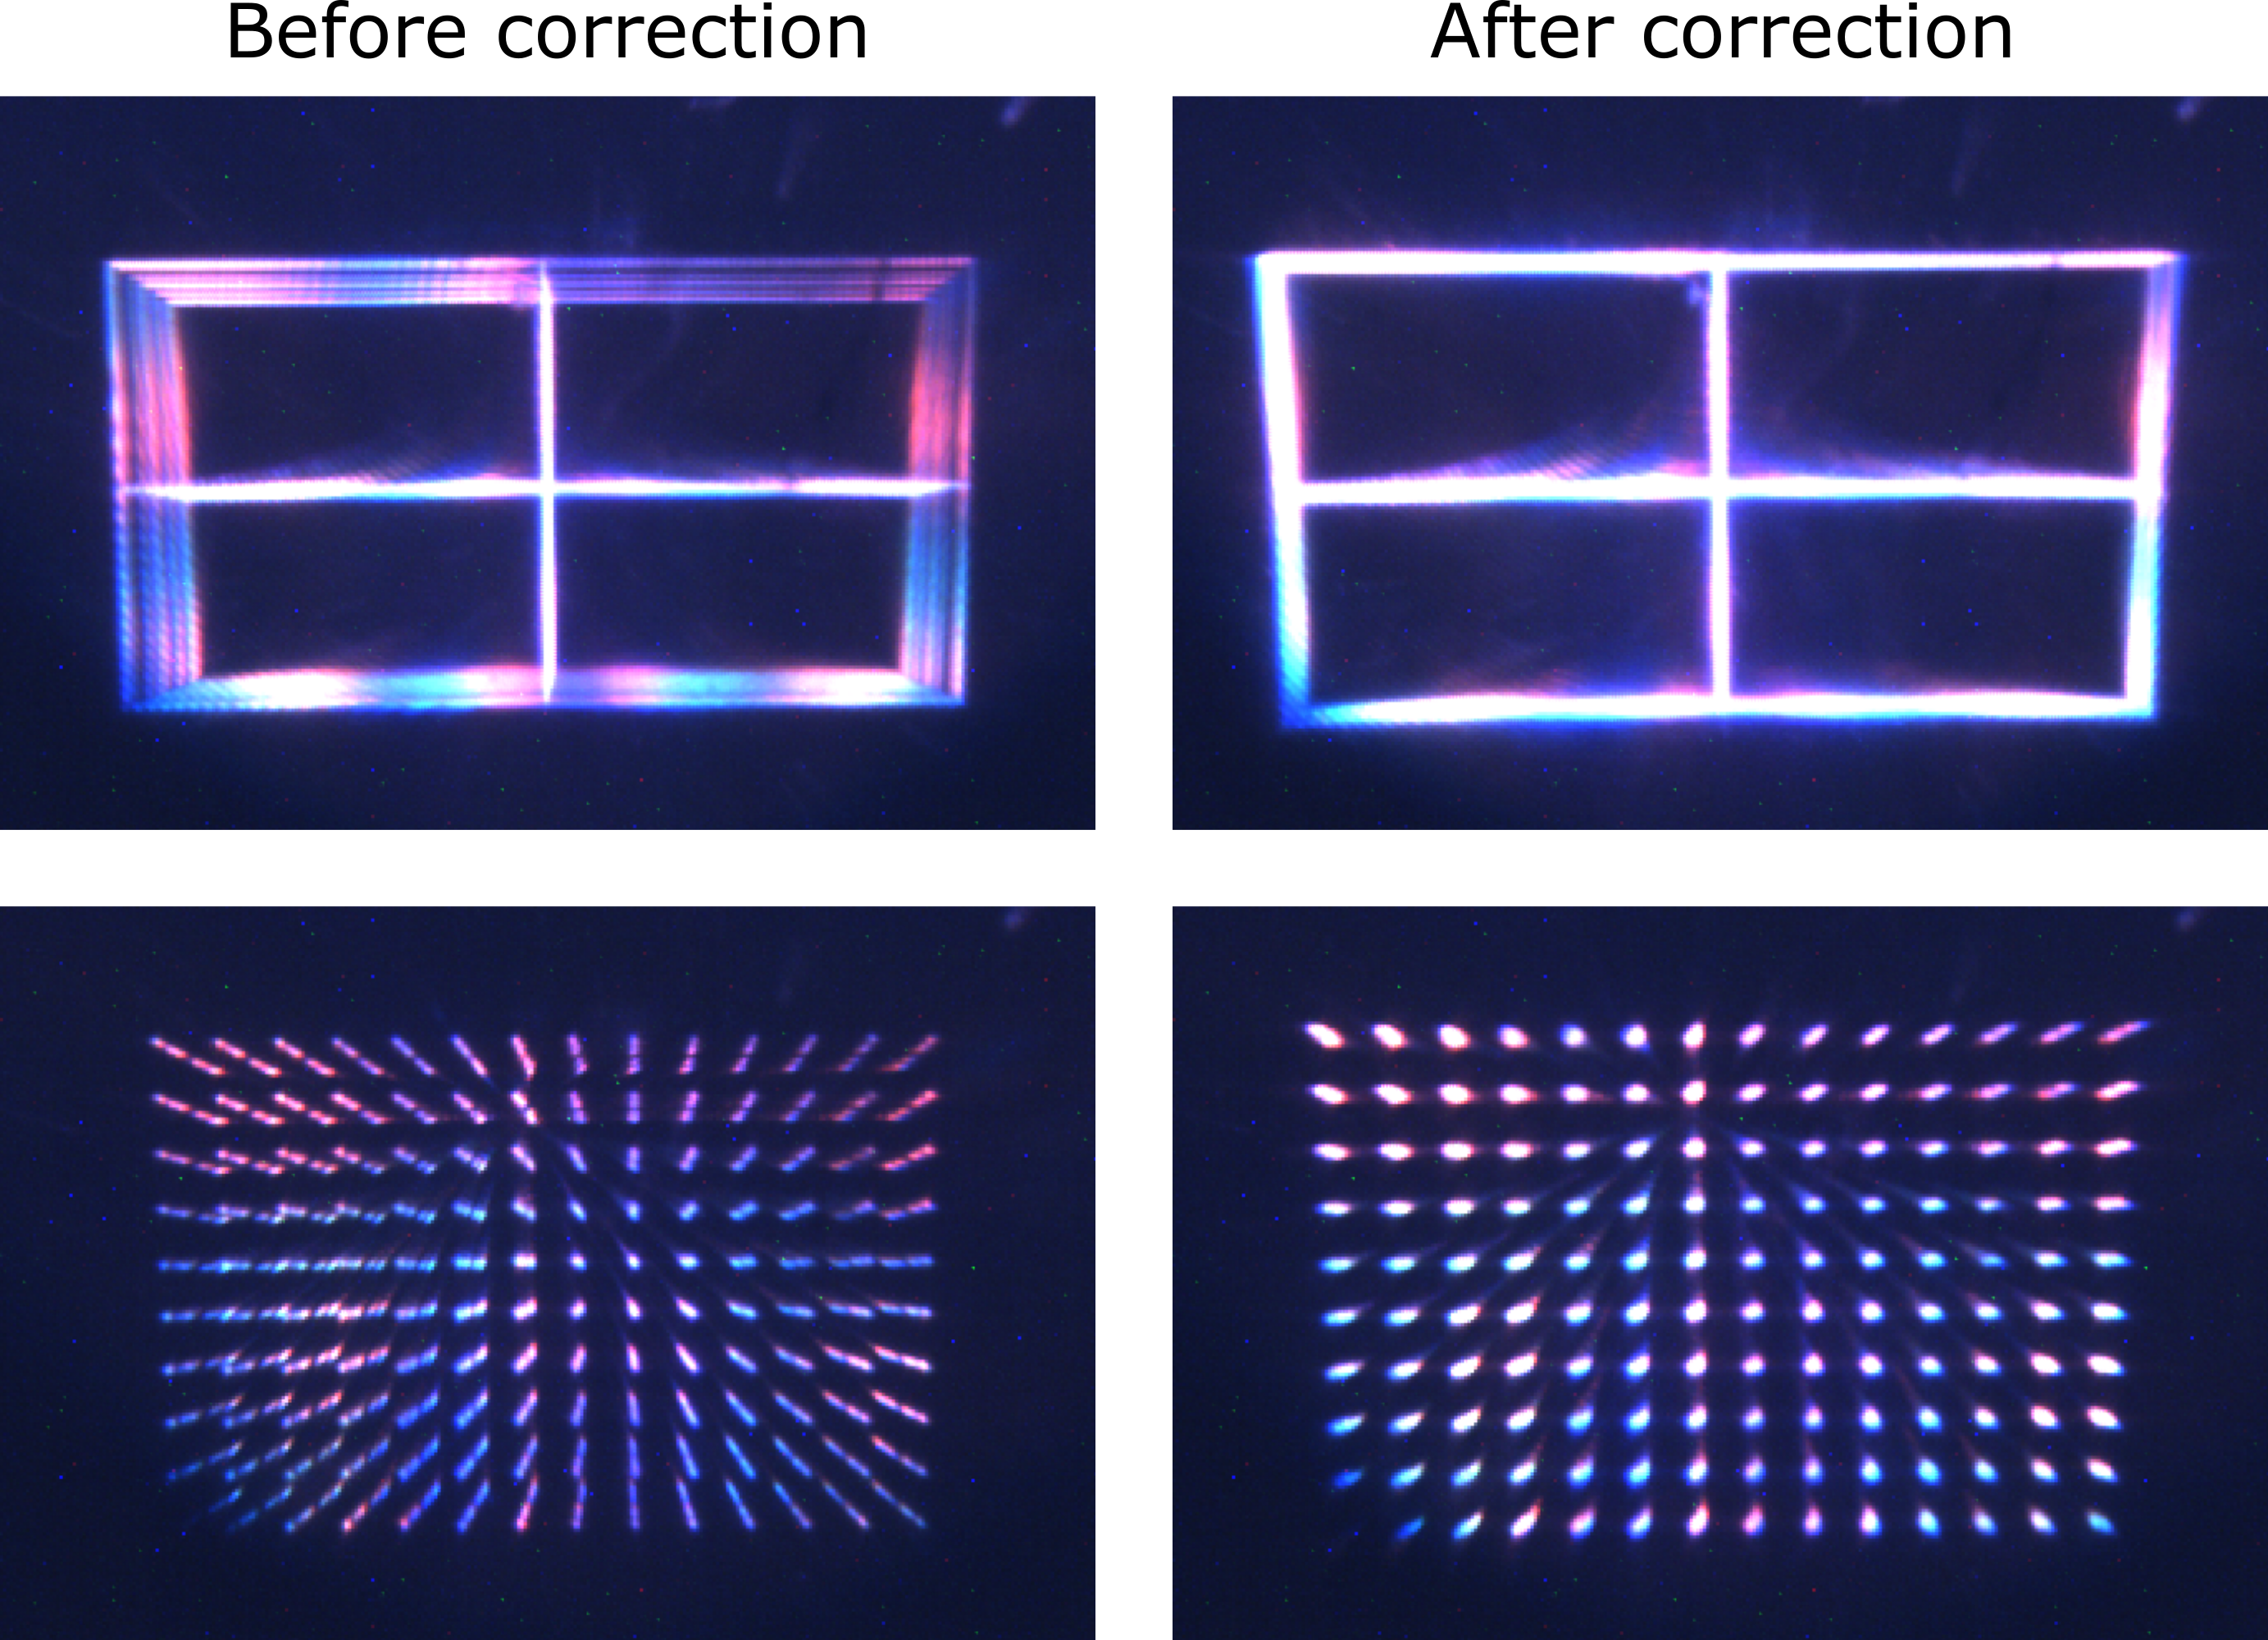
\includegraphics[width=\textwidth]{images/volumetric/distortion_correction/results}
\end{tabular}
\end{center}
\label{fig:volumetric:distortion_correction:results} 
\caption[Volumetric NED: Results of optical calibration and distortion correction]{Demonstration of our calibration and distortion-correction approach. For these images, the display is displaying a volume across a large depth-range (15 cm to 400 cm). To ensure that all the images in this large depth-range are clearly visible, the aperture of the camera was set to the smallest setting. The chromatic artifacts seem to occur only for this narrow aperture setting.}
\end{figure} 


Fig.~\ref{fig:volumetric:distortion_correction:results} (Top row) shows the before correction and after correction images for the calibration volume.
Notice how the rectangles do not line up in the before-calibration image, but they line up correctly in the after-calibration image. 
Another synthetic volume was generated composed of a point grid and placed at different depths. 
Fig.~\ref{fig:volumetric:distortion_correction:results} (Bottom row) shows the before and after images for the point-grid volume.
Notice how the points appear as lines in the before-calibration image but nearly appear as points in the after-calibration image.
Both images of Fig.~\ref{fig:volumetric:distortion_correction:results} were taken with a very narrow aperture camera so that the images at the different depths will appear clearly.
If we were to take these images with a wider aperture setting, only one of the depth-planes would be in-focus, and the others would be out-of-focus and appear very blurry preventing us from verifying whether our method works.
Images in Fig.~\ref{fig:volumetric:distortion_correction:results} appear to have severe chromatic artifacts, but this happens only when the aperture of the camera is very small; for a wider aperture setting, the chromatic artifacts are not present, and all visible pixels are bright white.
We do not fully understand the source of these chromatic artifacts. 

\subsection{Limitation of our approach}
Our approach does not address optical distortions that change across different lens cycles. To track optical distortions across lens cycles, we need a sophisticated lens tracking technology. Currently available lens tracking technologies are insufficient because they only track the focal length of the lens.
